\documentclass{standalone}
\usepackage{tikz}
\usetikzlibrary{patterns, positioning}
\usepackage[sfdefault]{ClearSans} %% option 'sfdefault' activates Clear Sans as the default text font
\usepackage[T1]{fontenc}

\begin{document}
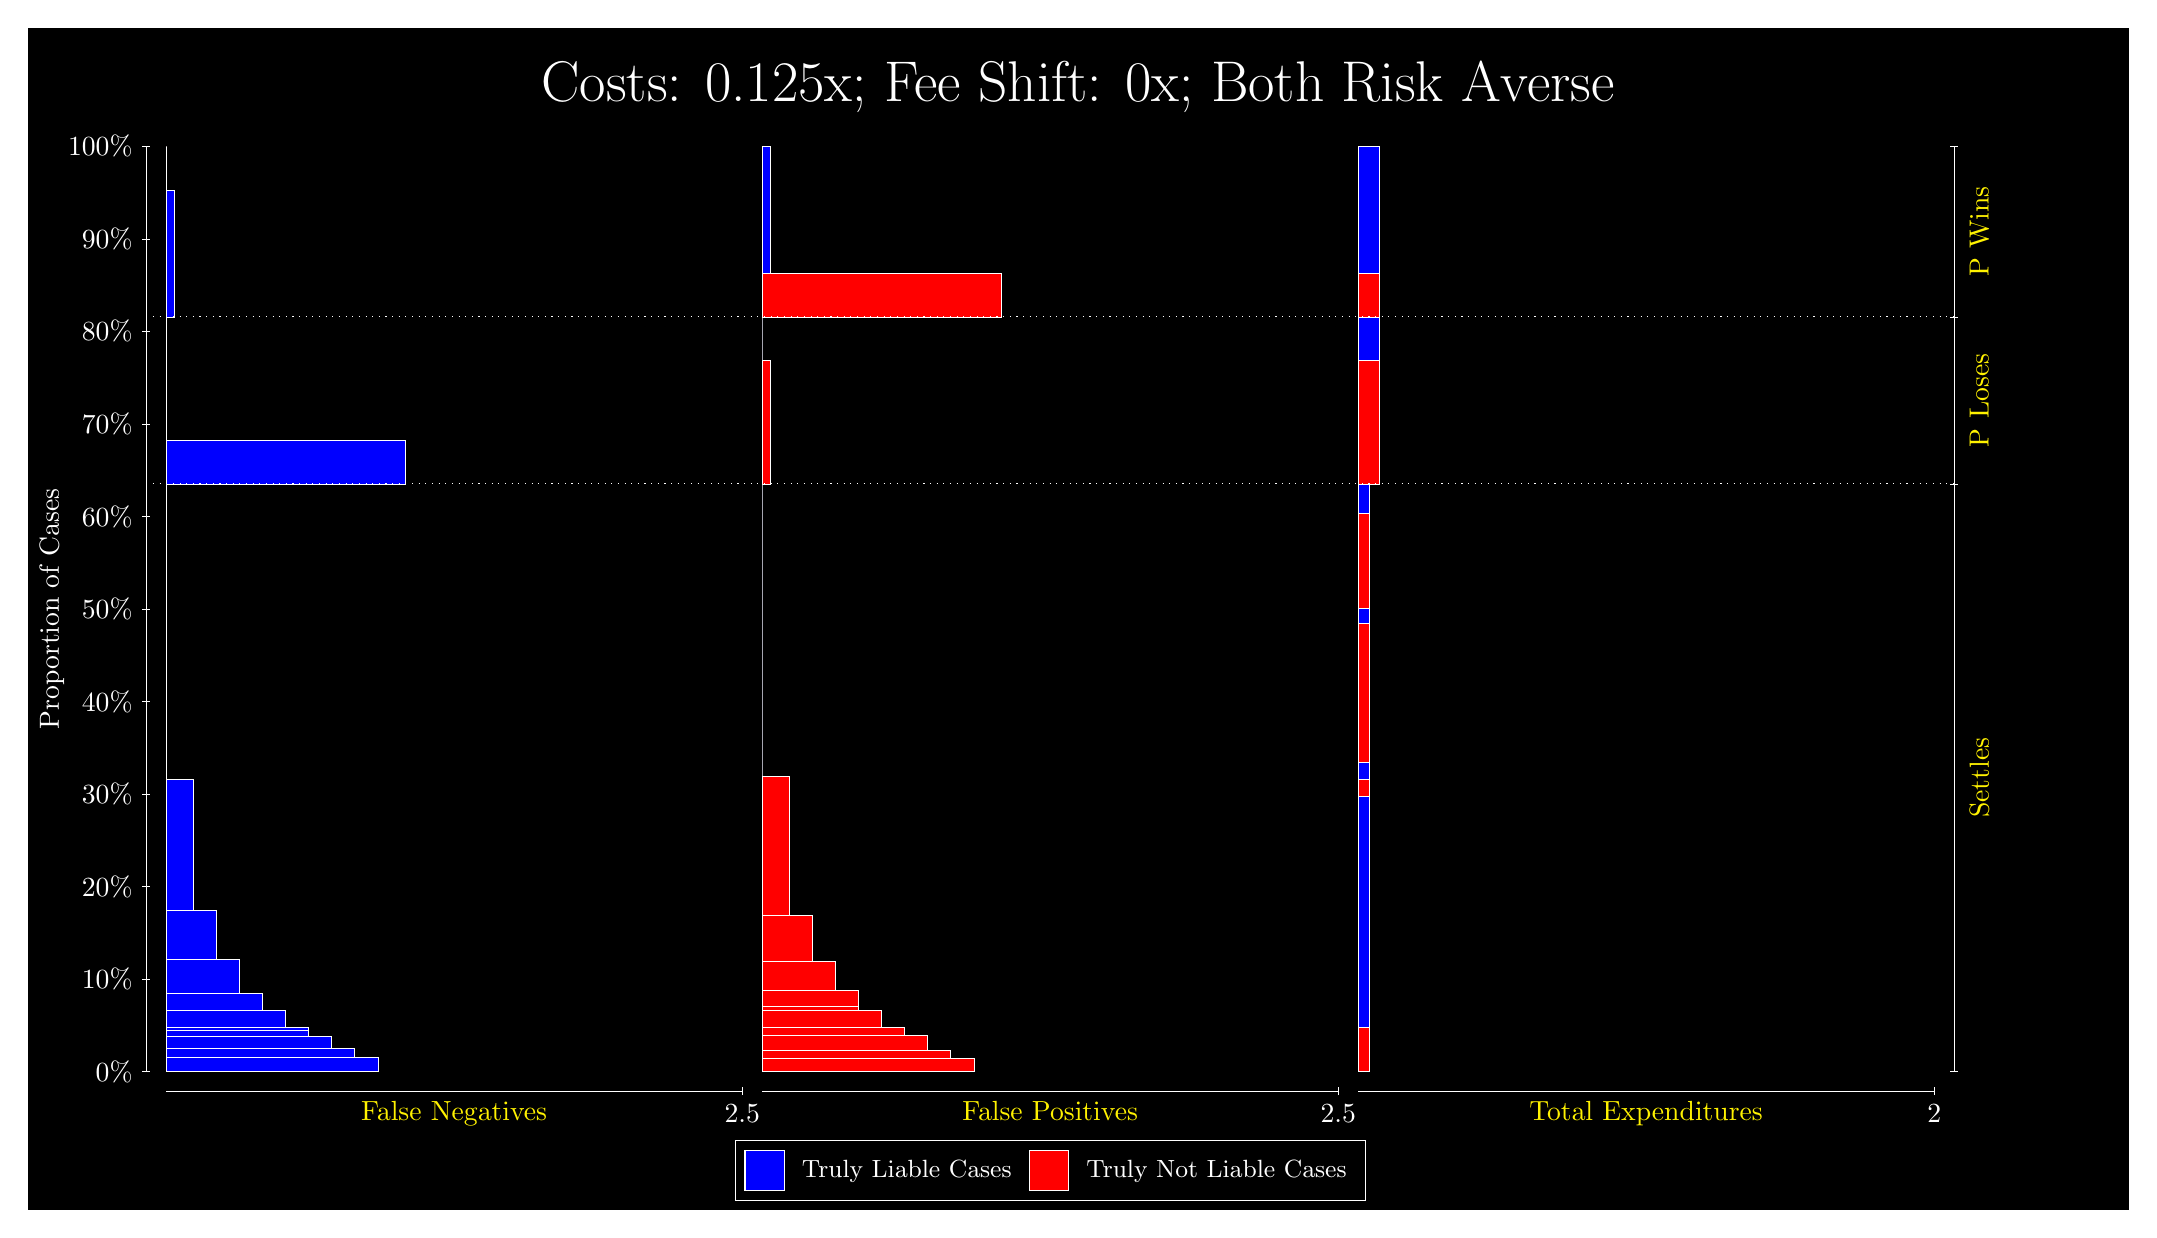
\begin{tikzpicture}
\draw[fill=black] (0,0) rectangle (26.667,15);
\draw[text=white] (0,13.5) rectangle (26.667,15) node[midway] {\huge Costs: 0.125x; Fee Shift: 0x; Both Risk Averse};
\draw[white, very thin] (1.5,1.75) -- (1.5,13.5);
\node[rotate=90, text=white, anchor=center] at (0.3, 7.625) {Proportion of Cases};
\draw[white, very thin] (1.45,1.75) -- (1.55,1.75);
\node[text=white, anchor=east] at (1.45, 1.75) {0\%};
\draw[white, very thin] (1.45,2.925) -- (1.55,2.925);
\node[text=white, anchor=east] at (1.45, 2.925) {10\%};
\draw[white, very thin] (1.45,4.1) -- (1.55,4.1);
\node[text=white, anchor=east] at (1.45, 4.1) {20\%};
\draw[white, very thin] (1.45,5.275) -- (1.55,5.275);
\node[text=white, anchor=east] at (1.45, 5.275) {30\%};
\draw[white, very thin] (1.45,6.45) -- (1.55,6.45);
\node[text=white, anchor=east] at (1.45, 6.45) {40\%};
\draw[white, very thin] (1.45,7.625) -- (1.55,7.625);
\node[text=white, anchor=east] at (1.45, 7.625) {50\%};
\draw[white, very thin] (1.45,8.8) -- (1.55,8.8);
\node[text=white, anchor=east] at (1.45, 8.8) {60\%};
\draw[white, very thin] (1.45,9.975) -- (1.55,9.975);
\node[text=white, anchor=east] at (1.45, 9.975) {70\%};
\draw[white, very thin] (1.45,11.15) -- (1.55,11.15);
\node[text=white, anchor=east] at (1.45, 11.15) {80\%};
\draw[white, very thin] (1.45,12.325) -- (1.55,12.325);
\node[text=white, anchor=east] at (1.45, 12.325) {90\%};
\draw[white, very thin] (1.45,13.5) -- (1.55,13.5);
\node[text=white, anchor=east] at (1.45, 13.5) {100\%};

\draw[white, very thin] (24.457,1.75) -- (24.457,13.5);
\draw[white, very thin] (24.407,1.75) -- (24.507,1.75);
\node[anchor=west] at (24.407, 1.75) {};
\draw[white, very thin] (24.407,9.2135) -- (24.507,9.2135);
\node[anchor=west] at (24.407, 9.2135) {};
\draw[white, very thin] (24.407,11.335) -- (24.507,11.335);
\node[anchor=west] at (24.407, 11.335) {};
\draw[white, very thin] (24.407,13.5) -- (24.507,13.5);
\node[anchor=west] at (24.407, 13.5) {};

\draw[white, very thin, fill=blue] (1.75,1.75) rectangle (4.4397,1.9321);
\draw[white, very thin, fill=blue] (1.75,1.9321) rectangle (4.1469,2.0403);
\draw[white, very thin, fill=blue] (1.75,2.0403) rectangle (3.8542,2.2005);
\draw[white, very thin, fill=blue] (1.75,2.2005) rectangle (3.5614,2.28);
\draw[white, very thin, fill=blue] (1.75,2.28) rectangle (3.5614,2.312);
\draw[white, very thin, fill=blue] (1.75,2.312) rectangle (3.2687,2.5256);
\draw[white, very thin, fill=blue] (1.75,2.5256) rectangle (2.9759,2.7472);
\draw[white, very thin, fill=blue] (1.75,2.7472) rectangle (2.6832,3.1812);
\draw[white, very thin, fill=blue] (1.75,3.1812) rectangle (2.3904,3.8008);
\draw[white, very thin, fill=blue] (1.75,3.8008) rectangle (2.0976,5.4604);
\draw[white, very thin, fill=red] (1.75,5.4604) rectangle (1.75,9.2135);
\draw[white, very thin, fill=blue] (1.75,9.2135) rectangle (4.7873,9.7697);
\draw[white, very thin, fill=red] (1.75,9.7697) rectangle (1.75,11.335);
\draw[white, very thin, fill=blue] (1.75,11.335) rectangle (1.8598,12.944);
\draw[white, very thin, fill=red] (1.75,12.944) rectangle (1.75,13.5);
\draw[white, very thin, fill=red] (9.3189,1.75) rectangle (12.009,1.9148);
\draw[white, very thin, fill=red] (9.3189,1.9148) rectangle (11.716,2.0261);
\draw[white, very thin, fill=red] (9.3189,2.0261) rectangle (11.423,2.2121);
\draw[white, very thin, fill=red] (9.3189,2.2121) rectangle (11.13,2.3142);
\draw[white, very thin, fill=red] (9.3189,2.3142) rectangle (10.838,2.5298);
\draw[white, very thin, fill=red] (9.3189,2.5298) rectangle (10.545,2.5793);
\draw[white, very thin, fill=red] (9.3189,2.5793) rectangle (10.545,2.7786);
\draw[white, very thin, fill=red] (9.3189,2.7786) rectangle (10.252,3.1544);
\draw[white, very thin, fill=red] (9.3189,3.1544) rectangle (9.9593,3.7337);
\draw[white, very thin, fill=red] (9.3189,3.7337) rectangle (9.6665,5.5031);
\draw[white, very thin, fill=blue] (9.3189,5.5031) rectangle (9.3189,9.2135);
\draw[white, very thin, fill=red] (9.3189,9.2135) rectangle (9.4287,10.779);
\draw[white, very thin, fill=blue] (9.3189,10.779) rectangle (9.3189,11.335);
\draw[white, very thin, fill=red] (9.3189,11.335) rectangle (12.356,11.892);
\draw[white, very thin, fill=blue] (9.3189,11.892) rectangle (9.4287,13.5);
\draw[white, very thin, fill=red] (16.888,1.75) rectangle (17.025,2.3142);
\draw[white, very thin, fill=blue] (16.888,2.3142) rectangle (17.025,5.2489);
\draw[white, very thin, fill=red] (16.888,5.2489) rectangle (17.025,5.4645);
\draw[white, very thin, fill=blue] (16.888,5.4645) rectangle (17.025,5.6781);
\draw[white, very thin, fill=red] (16.888,5.6781) rectangle (17.025,7.4476);
\draw[white, very thin, fill=blue] (16.888,7.4476) rectangle (17.025,7.6297);
\draw[white, very thin, fill=red] (16.888,7.6297) rectangle (17.025,8.8336);
\draw[white, very thin, fill=blue] (16.888,8.8336) rectangle (17.025,9.2135);
\draw[white, very thin, fill=red] (16.888,9.2135) rectangle (17.162,10.779);
\draw[white, very thin, fill=blue] (16.888,10.779) rectangle (17.162,11.335);
\draw[white, very thin, fill=red] (16.888,11.335) rectangle (17.162,11.892);
\draw[white, very thin, fill=blue] (16.888,11.892) rectangle (17.162,13.5);
\draw[white, dotted] (1.5,9.2135) -- (24.457,9.2135);
\draw[white, dotted] (1.5,11.335) -- (24.457,11.335);
\draw[white, very thin] (1.75,1.5) -- (9.0689,1.5);
\node[text=yellow, anchor=north] at (5.4094, 1.5) {False Negatives};
\draw[white, very thin] (9.0689,1.45) -- (9.0689,1.55);
\node[text=white, anchor=north] at (9.0689, 1.45) {2.5};

\draw[white, very thin] (9.3189,1.5) -- (16.638,1.5);
\node[text=yellow, anchor=north] at (12.978, 1.5) {False Positives};
\draw[white, very thin] (16.638,1.45) -- (16.638,1.55);
\node[text=white, anchor=north] at (16.638, 1.45) {2.5};

\draw[white, very thin] (16.888,1.5) -- (24.207,1.5);
\node[text=yellow, anchor=north] at (20.547, 1.5) {Total Expenditures};
\draw[white, very thin] (24.207,1.45) -- (24.207,1.55);
\node[text=white, anchor=north] at (24.207, 1.45) {2};

\node[text=yellow, centered, rotate=90] at (24.777, 5.4818) {Settles};
\node[text=yellow, centered, rotate=90] at (24.777, 10.274) {P Loses};
\node[text=yellow, centered, rotate=90] at (24.777, 12.418) {P Wins};

\draw (12.978300999999998,1.5) node[draw=none] (baseCoordinate) {};
\begin{scope}[align=center]
        \matrix[scale=0.5, draw=white, below=0.5cm of baseCoordinate, nodes={draw}, column sep=0.1cm]{
            \node[rectangle, draw, minimum width=0.5cm, minimum height=0.5cm, fill=blue] {}; &
            \node[draw=none, font=\small, text=white] (B) {Truly Liable Cases}; &
            \node[rectangle, draw, minimum width=0.5cm, minimum height=0.5cm, fill=red] {}; &
            \node[draw=none, font=\small, text=white] (B) {Truly Not Liable Cases}; \\
            };
\end{scope}

\end{tikzpicture}
\end{document}